

\begin{frame}{Longest Common Subsequence}
\only <1>
{
From the two given sequences, we have to find a subsequence that is present in both of them and is the longest.

	\begin{figure}[h]
	% \captionsetup{labelformat=empty}
	% \caption{A common example to compare DNA strings}
	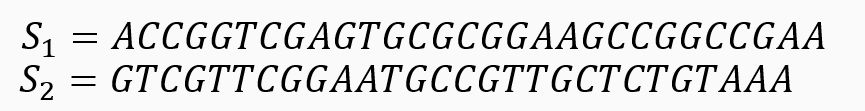
\includegraphics[width=0.5\textwidth]{Assets/LCS_1.png}
	\label{fig:1}
\end{figure}

}
\only<2>
{
\begin{figure}[h]
	% \captionsetup{labelformat=empty}
	% \caption{A common example to compare DNA strings}
	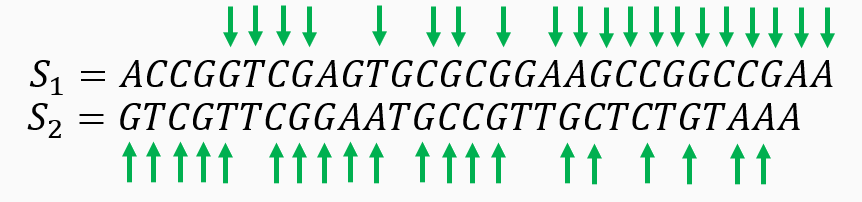
\includegraphics[width=0.5\textwidth]{Assets/LCS_2.png}
	\label{fig:1}
	\end{figure}

\centering
% \textbf{Helps us to compare how similar the two DNA strands are. }
\begin{figure}[h]
	% \captionsetup{labelformat=empty}
	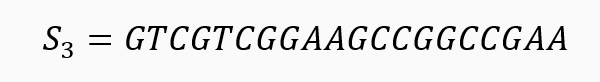
\includegraphics[width=0.5\textwidth]{Assets/LCS_final.png}
	\label{fig:1}
\end{figure}
}
	
\end{frame}
